\section{System Identification}

Consider our system of a parachute attached to a spherical mass by a string being thrown through the air. How can we model this system? The answer may seem obvious depending on your physics background, but we claim that nothing is obvious.\footnote{Any problem worth studying will not have an obvious answer. If the answer seems obvious, question your assumptions.}

First it's important to identify what properties of the system we're actually interested in. Here we've decided we're interested in modeling the trajectory of the center of mass of the ball. Some things we aren't interested in are the motion of the parachute, the mass of the ball, the elasticity of the ball, the color of the ball, the temperature of the room, the location of the moon in relation to the Earth, what you had for breakfast, etc. 

Everything in the universe is connected\footnote{This is readily apparent by considering gravity or electromagnetism.} and where we choose to draw the line may seem arbitrary. Obviously we won't be modeling every atom of our system and all the forces they're experiencing, and yet there are still a handful of reasonable options:

\begin{itemize}
\item Point Mass, No Drag

The ball-chute system could be modeled as a single point mass in a vacuum traveling on a parabolic trajectory. This would certainly lead to inaccuracies once a large parachute is used, but it may be a decent approximation in low-drag scenarios. \footnote{ADD FIGURE: Freebody diagram}

\item Point Mass, Linear Drag 

The simplest way to incorporate air resistance into our model is as a force proportional to the velocity of the ball.\footnote{ADD FIGURE: Freebody diagram}

\item Point Mass, Velocity-Squared Drag

At higher velocities, the effect of drag tends to depart from a simple linear relationship towards a velocity squared relationship

\item Multi-body System

The intention of the parachute was simply to increase the drag of the ball, but it's certainly more complicated than that in reality. A more accurate model of the system would represent the ball and parachute as separate bodies, potentially even modeling the off-center attachment point of the parachute. 

\end{itemize}

With all these options available to us, we refer to the following principle: keep it simple. We don't want to over-complicate things unless we know that we have to. We don't want to waste effort optimizing something until we know it's a bottleneck. Following this principle, we'll start by modeling our system as a point mass with no drag. There are several benefits to following this approach. 

First, we know what behavior to expect from this model. The trajectory is a simple parabola. This will make it easier to spot coding mistakes by providing us with a known output. We're going to write a lot of code, so anything to help minimize the chances for bugs to slip through is appreciated. 

Second, the anticipated failure of the parabolic model will serve as our evidence that it's worth investing more time into developing the linear drag model. If we're exercising our engineering skills, pretending this project is analogous to a more ambitious program, then this evidence would be highly valuable to our stakeholders in justifying why we should invest in the more complicated version. In a real setting, it's possible that we may have incorrect assumptions and this simple version may end up fully satisfying our system requirements, putting us ahead of schedule and under budget.

Finally, even though we already know we'll be moving on to the linear drag model, without some baseline to compare against we can't actually \textit{know} if the linear drag model is doing any better than the parabolic model. We'd just be a bunch of speculating nerds claiming it's better based on \textit{a priori} mathematics, and math is just a bunch of numbers that I don't understand. By actually implementing the two versions of the model, we can compare them back to back. 

\subsection{Generic Model Structure}

We consider now the mathematical structure of the model. What exactly should the model describe? Well it's the trajectory, but what as a function of what? In what type of coordinates? Polar? Cartesian? Perhaps separate component functions?

We will represent our trajectory in a generalized form: position vector as a function of time ${\bf r}(t) \in \mathbb{R}^n, n = 2, t \in [0,t_{impact}]$. Using this very generic notation allows us the most flexibility for extending our work to more complicated systems in the future. We will also want to include the velocity and acceleration of the projectile included in the model. These quantities are derived from the position, and you could therefore argue they're redundant to include as part of the model structure, but explicitly listing them as a requirement here will lead to code design choices later that will make the model easier to use.

Additionally, we will call out the time of impact $t_{impact} \in \mathbb{R} > 0$ to be part of the model structure.\footnote{Within the scope of this project, the time of impact is simply when the vertical component of the position function = 0. However, defining it as a model parameter means we can change how it's computed in the future, allowing for more complicated collision intersection calculations.}

Generic model structure:
% Parabolic Model
\begin{align*}
Model =
\begin{cases} 
\ddot{\bf r}(t) & acceleration \\
\dot{\bf r}(t) & velocity \\
{\bf r}(t) & position \\
t_{impact}
\end{cases}
\end{align*}

\subsection{Parabolic Model}
We now present the parabolic model, which is simply the equations of motion for an object in free-fall. The derivation of these equations is given in the appendix\footnote{TODO}.

\begin{align*}
Model_{parabolic} = 
\begin{cases}
\ddot{\bf r}(t) = -g\hat{y} \\
\dot{\bf r}(t) = -g\hat{y}t + \dot{\bf r}_0 \\
{\bf r}(t) = -\frac12g\hat{y}t^2 + \dot{\bf r}_0t + {\bf r}_0 \\
t_{impact} = t > 0\text{ where }{\bf r}_y(t) = 0
\end{cases}
\end{align*}

where $g=9.81m/s^2$ is the acceleration due to gravity, ${\bf r}_0$ is the initial position, $\dot{\bf r}_0$ is the initial velocity, and $\hat{y}$ is the unit vector in the upwards vertical direction. A portion of the code implementation of this model is shown in Fig.~\ref{fig:model_matlab_code_nodrag}.

\begin{figure}[t]
\centering
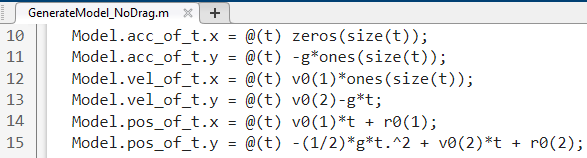
\includegraphics[width=0.75\linewidth]{images/model_matlab_code_nodrag.png}
\caption{\label{fig:model_matlab_code_nodrag} Equations of motion for an object in freefall implemented in MATLAB. Full code available on GitHub.}
\end{figure}






